\chapter{Electrode Kinetics and Electroanalysis}\label{ch:b3:electrode-kinetics}

A drop of blood on a strip of plastic, five seconds, a number: the glucose
meter that millions of people use several times a day is an electrochemical
cell, and what it measures is not a voltage but a current. An \omterm{def:b3:complex-kinetics:enzyme}{enzyme} oxidises
the glucose, a dissolved iron complex carries the electrons to a carbon
electrode, and the current that flows is set by how fast that complex diffuses
to the electrode, hence by its concentration. This chapter explains why
electrons cross an interface fast or slowly (the \omterm{thm:b3:electrode-kinetics:butler-volmer}{Butler--Volmer equation}), how
mass transport limits the current, and how \omterm{def:b3:electrode-kinetics:cv}{cyclic voltammetry} and the other
electroanalytical methods turn currents into concentrations, rate constants
and mechanisms.

\begin{recall}
The Year 1 volume defined the electrode potential, the standard potential, the
Nernst equation, reference electrodes and half-cells. The Year 2 volume
introduced current--potential curves with their anodic and cathodic currents,
working and counter electrodes, overpotentials, fast and slow systems, the
diffusion layer and the limiting current; activity coefficients and ionic
strength; calibration curves, the standard-addition method and the limit of
detection. \Cref{ch:b3:rate-theories} gave \omterm{def:b3:rate-theories:tst}{transition-state theory}. From
physics: Fick's laws of diffusion, Poisson's equation and capacitors.
\end{recall}

\begin{omfigure}
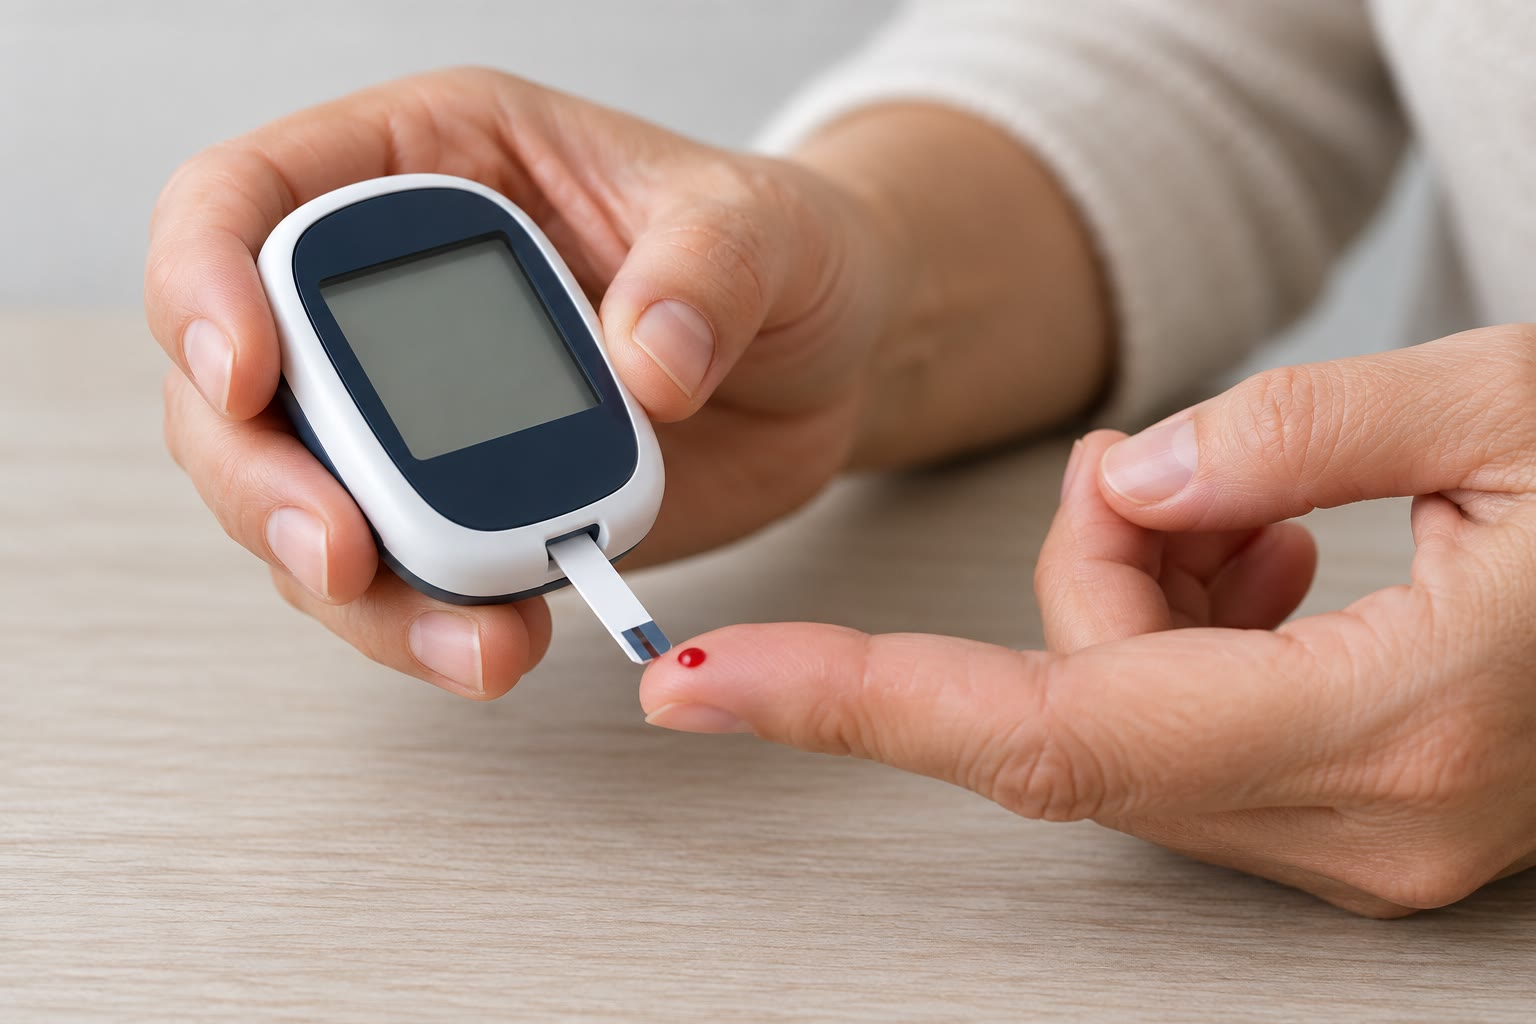
\includegraphics[width=0.6\linewidth]{images/book4/ai/b3-15-glucose-meter.jpg}

{\small A blood-glucose meter: the strip carries a tiny three-electrode cell
with an \omterm{def:b3:complex-kinetics:enzyme}{enzyme} and a redox mediator; the meter applies a potential and reads a
current.}
\end{omfigure}

\section{The electrode--solution interface}

A metal plunged into an electrolyte solution carries a surface charge, and the
solution answers with an equal and opposite charge made of an excess of ions
of one sign. The two layers of charge form a capacitor of molecular thickness.

\begin{definition}[Electrical double layer]\label{def:b3:electrode-kinetics:double-layer}
The \emph{electrical double layer}\index{electrical double layer} is the
arrangement of charge at an electrode--solution interface: the charge on the
metal and the compensating ionic charge in the solution. Its compact part, the
\emph{Helmholtz layer}\index{Helmholtz layer}, is the layer of ions and solvent
molecules in contact with the surface; its \emph{diffuse layer}\index{diffuse
layer} is the region beyond, where thermal motion spreads the excess ions over
a distance of the order of the \emph{Debye length}\index{Debye length} $\kappa^{-1}$. The
\emph{double-layer capacitance}\index{double-layer capacitance} $C_{\mathrm{dl}}$ is the charge
stored per unit area per volt of potential across the interface.
\end{definition}

\begin{proposition}[Debye length]\label{prop:b3:electrode-kinetics:debye-length}
In a solution of ionic strength $I$ (in \unit{mol.m^{-3}}) and relative permittivity
$\varepsilon_r$, a small potential $\varphi_0$ at the electrode decays into the solution as
$\varphi = \varphi_0\eu^{-\kappa x}$, with
\[
  \kappa^{-1} = \sqrt{\frac{\varepsilon_r\varepsilon_0RT}{2F^2I}} .
\]
\end{proposition}

\begin{proof}
Poisson's equation (from physics) relates the potential to the charge density:
$\dd^2\varphi/\dd x^2 = -\rho/\varepsilon_r\varepsilon_0$. Each ion obeys the \omterm{def:b3:partition-functions:boltzmann}{Boltzmann distribution} in the
potential: $c_i = c_i^{\circ}\eu^{-z_iF\varphi/RT}$, so $\rho = F\sum_iz_ic_i^{\circ}\eu^{-z_iF\varphi/RT}$. For $F\varphi \ll RT$,
$\eu^{-z_iF\varphi/RT} \approx 1 - z_iF\varphi/RT$; the zero-order terms cancel by electroneutrality,
and $\rho \approx -(F^2/RT)\sum_iz_i^2c_i^{\circ}\,\varphi = -(2F^2I/RT)\varphi$. Hence $\dd^2\varphi/\dd x^2 = \kappa^2\varphi$, whose
solution vanishing far away is $\varphi_0\eu^{-\kappa x}$.
\end{proof}

\begin{example}[The thickness of the double layer]\label{ex:b3:electrode-kinetics:debye}
% ledger: eps:H2O.25C, const:eps0, const:F, const:R
In water at \qty{298.15}{K} ($\varepsilon_r = 78.4$) with \qty{0.10}{mol/L} of a 1:1 salt ($I = \qty{100}{mol.m^{-3}}$),
$\kappa^{-1} = \sqrt{78.4 \times \num{8.854e-12} \times 2479/(2 \times 96\,485^2 \times 100)} = \qty{0.96}{nm}$; at \qty{1.0}{mmol/L},
ten times more. A \omterm{def:b3:electrode-kinetics:transport}{supporting electrolyte} compresses the \omterm{def:b3:electrode-kinetics:double-layer}{diffuse layer} to a few
molecular diameters.
\end{example}

The \omterm{def:b3:electrode-kinetics:double-layer}{diffuse layer} behaves as a capacitor whose plates are $\kappa^{-1}$ apart: its
capacitance per unit area at low potential is $\varepsilon_r\varepsilon_0\kappa$ (the Gouy--Chapman
result; its dependence on the potential is admitted). In series with the
compact \omterm{def:b3:electrode-kinetics:double-layer}{Helmholtz layer}, it gives the measured $C_{\mathrm{dl}}$, of the order of tens of
microfarads per square centimetre (the Stern model). Whenever the potential changes, this capacitor
charges: a scan at $v$ volts per second draws a charging current $C_{\mathrm{dl}}Av$ that
carries no chemistry and adds to every voltammetric measurement.

\begin{omfigure}
\begin{tikzpicture}[font=\small, >=Stealth]
  \fill[black!25] (-1.0,0) rectangle (0,3.2);
  \node[rotate=90] at (-0.5,1.6) {metal};
  \foreach \y in {0.3,0.8,...,2.9}{\node[font=\scriptsize] at (-0.15,\y) {$-$};}
  \foreach \y in {0.35,0.95,1.55,2.15,2.75}{\draw[omDef, fill=omDef!20] (0.3,\y) circle (0.18); \node[font=\scriptsize] at (0.3,\y) {$+$};}
  \draw[black!50, dashed] (0.55,0) -- (0.55,3.2);
  \node[font=\scriptsize, anchor=south, align=center] at (0.45,3.25) {Helmholtz\\ plane};
  \foreach \x/\y/\s in {1.1/0.6/+, 1.4/2.2/+, 1.9/1.3/+, 2.3/2.7/-, 2.6/0.5/+, 3.1/1.8/+, 3.5/0.9/-, 3.9/2.4/+, 4.4/1.4/-, 4.8/0.4/+, 5.1/2.8/-, 5.4/1.9/+}{
    \draw[black!60, fill=white] (\x,\y) circle (0.15); \node[font=\scriptsize] at (\x,\y) {$\s$};}
  \node[font=\scriptsize, anchor=south] at (3.2,3.25) {diffuse layer};
  \draw[->] (0,-2.1) -- (6.0,-2.1) node[anchor=north east] {$x$};
  \draw[->] (0,-2.1) -- (0,-0.3) node[anchor=east] {$|\varphi|$};
  \draw[omThm, thick] (0,-0.5) -- (0.55,-1.0) plot[domain=0.55:5.8, samples=40] (\x,{-2.1+1.1*exp(-(\x-0.55)/1.2)});
  \draw[black!40, dashed] (0.55,-2.1) -- (0.55,-0.4);
  \node[omThm, anchor=south west] at (1.3,-1.6) {$|\varphi(x)|$};
  \draw[<->, black!60] (0.55,-2.5) -- (1.75,-2.5) node[midway, below, font=\scriptsize] {$\sim\kappa^{-1}$};
\end{tikzpicture}

{\small The \omterm{def:b3:electrode-kinetics:double-layer}{electrical double layer} (Gouy--Chapman--Stern model, schematic): a
negatively charged metal, a compact layer of cations at the Helmholtz plane,
and a \omterm{def:b3:electrode-kinetics:double-layer}{diffuse layer} where cations outnumber anions over a few \omterm{def:b3:electrode-kinetics:double-layer}{Debye lengths}.
Below, the size of the potential (negative, like the charge of the metal) falls
linearly across the compact layer, then exponentially in the \omterm{def:b3:electrode-kinetics:double-layer}{diffuse layer}.}
\end{omfigure}

\section{Electron-transfer kinetics}

Consider the reduction $\mathrm{O} + n\,\mathrm{e}^- \to \mathrm{R}$ at an electrode held at the potential $E$,
whose equilibrium potential for the bulk solution would be $E_{\mathrm{eq}}$. The
overpotential is $\eta = E - E_{\mathrm{eq}}$.

\begin{definition}[Exchange current density, transfer coefficient, standard rate constant]\label{def:b3:electrode-kinetics:exchange}
At equilibrium the anodic and cathodic currents are equal and opposite; their
common magnitude per unit area is the \emph{exchange current
density}\index{exchange current density} $j_0$. The \emph{transfer
coefficient}\index{transfer coefficient} $\alpha$ ($0 < \alpha < 1$) is the fraction of the
electrical energy $nF\eta$ that lowers the barrier of the cathodic reaction. The
\emph{standard rate constant}\index{standard rate constant} $k^\circ$ is the common
value of the cathodic and anodic rate constants at the formal potential $E^{\circ\prime}$.
\end{definition}

\begin{theorem}[Butler--Volmer equation]\label{thm:b3:electrode-kinetics:butler-volmer}
If the surface concentrations equal the bulk ones (no mass-transport
limitation), the current density at overpotential $\eta$ is, counting anodic
currents positive,
\[
  j = j_0\bigl[\eu^{(1 - \alpha)f\eta} - \eu^{-\alpha f\eta}\bigr], \qquad f = \frac{nF}{RT}.
\]
This is the \emph{Butler--Volmer equation}\index{Butler--Volmer equation}.
\end{theorem}

\begin{proof}
By \omterm{def:b3:rate-theories:tst}{transition-state theory} the cathodic and anodic rate constants are
$k_{\mathrm c} = A\eu^{-\Delta G_{\mathrm c}^{\ddagger}/RT}$ and $k_{\mathrm a} = A\eu^{-\Delta G_{\mathrm a}^{\ddagger}/RT}$. Changing the electrode potential by $\delta E$
changes the Gibbs energy of the reaction $\mathrm{O} + n\,\mathrm{e}^- \to \mathrm{R}$ by $nF\,\delta E$ (the electrons
in the metal gain $-nF\,\delta E$ of electrical energy). Assume, to first order, that a
fraction $\alpha$ of this change goes into the cathodic barrier and the rest into the
anodic one: $\Delta G_{\mathrm c}^{\ddagger} \to \Delta G_{\mathrm c}^{\ddagger} + \alpha nF\,\delta E$, $\Delta G_{\mathrm a}^{\ddagger} \to \Delta G_{\mathrm a}^{\ddagger} - (1 - \alpha)nF\,\delta E$. Measuring $\delta E$
from the equilibrium potential, where the two currents are both $j_0$ in
magnitude, gives $j_{\mathrm c} = j_0\eu^{-\alpha f\eta}$ and $j_{\mathrm a} = j_0\eu^{(1 - \alpha)f\eta}$; the net current is their
difference.
\end{proof}

\begin{corollary}[Charge-transfer resistance]\label{cor:b3:electrode-kinetics:linear}
For $|\eta| \ll RT/nF$, $j = j_0f\eta$: the interface behaves as a resistance
$R_{\mathrm{ct}} = RT/(nFi_0)$, with $i_0 = j_0A$.
\end{corollary}

\begin{proof}
Expand both exponentials to first order: $j = j_0[(1 - \alpha)f\eta + \alpha f\eta] = j_0f\eta$; then
$\eta/i = 1/(fi_0)$.
\end{proof}

\begin{corollary}[Tafel equation]\label{cor:b3:electrode-kinetics:tafel}
For $\eta \ll -RT/nF$ (a strongly cathodic overpotential), the anodic term is
negligible and
\[
  \eta = \frac{2.303\,RT}{\alpha nF}\bigl(\log j_0 - \log|j|\bigr):
\]
$\log|j|$ is linear in $\eta$, with a slope of $1/(\text{\qty{118}{mV}})$ per decade at \qty{298}{K} for $\alpha = 0.5$, $n =
1$. This is the \emph{Tafel equation}\index{Tafel equation}.
\end{corollary}

\begin{proof}
$|j| = j_0\eu^{-\alpha f\eta}$, so $\ln|j| = \ln j_0 - \alpha f\eta$; convert to decimal logarithms.
\end{proof}

\begin{definition}[Charge-transfer resistance, Tafel slope]\label{def:b3:electrode-kinetics:charge-transfer}
The \emph{charge-transfer resistance}\index{charge-transfer resistance} of an
electrode is $R_{\mathrm{ct}} = (\partial\eta/\partial i)_{\eta = 0}$. The \emph{Tafel slope}\index{Tafel slope}
is the change of overpotential per decade of current in the Tafel region,
$2.303\,RT/\alpha nF$.
\end{definition}

\begin{omfigure}
\begin{tikzpicture}
\begin{axis}[name=bv, omcv, width=0.47\linewidth, height=5.4cm, xmin=-300, xmax=300, ymin=-40, ymax=40,
  xlabel={$\eta$ / mV}, ylabel={$j/j_0$},
  legend style={font=\scriptsize, draw=none, at={(0.03,0.97)}, anchor=north west}, legend cell align=left]
\addplot[omDef, thick] table[x=eta_mV, y=a3] {figdata/out/bachelor-3-butler-volmer.dat};
\addplot[black, thick] table[x=eta_mV, y=a5] {figdata/out/bachelor-3-butler-volmer.dat};
\addplot[omThm, thick] table[x=eta_mV, y=a7] {figdata/out/bachelor-3-butler-volmer.dat};
\legend{$\alpha = 0.3$, $\alpha = 0.5$, $\alpha = 0.7$}
\draw[black!30] (axis cs:-300,0) -- (axis cs:300,0) (axis cs:0,-40) -- (axis cs:0,40);
\end{axis}
\begin{axis}[at={(bv.east)}, anchor=west, xshift=1.2cm, omcv, width=0.47\linewidth, height=5.4cm,
  xmin=-300, xmax=300, ymin=-1.5, ymax=4, xlabel={$\eta$ / mV}, ylabel={$\log|j/j_0|$},
  unbounded coords=jump]
\addplot[omDef, thick] table[x=eta_mV, y=l3] {figdata/out/bachelor-3-butler-volmer.dat};
\addplot[black, thick] table[x=eta_mV, y=l5] {figdata/out/bachelor-3-butler-volmer.dat};
\addplot[omThm, thick] table[x=eta_mV, y=l7] {figdata/out/bachelor-3-butler-volmer.dat};
\draw[black!40, dashed] (axis cs:-300,2.54) -- (axis cs:0,0);
\draw[black!50] (axis cs:-200,1.85) -- (axis cs:-120,3.3) node[anchor=south, font=\scriptsize, inner sep=1pt] {slope $1/(\qty{118}{mV})$};
\end{axis}
\end{tikzpicture}

{\small The \omterm{thm:b3:electrode-kinetics:butler-volmer}{Butler--Volmer equation} ($n = 1$, \qty{298}{K}) for three \omterm{def:b3:electrode-kinetics:exchange}{transfer
coefficients}. Left: the current is linear in $\eta$ near equilibrium (the
\omterm{def:b3:electrode-kinetics:charge-transfer}{charge-transfer resistance}) and exponential beyond; $\alpha$ makes it asymmetric.
Right: the Tafel plot, whose straight branches extrapolate to $\log|j/j_0| = 0$
at $\eta = 0$; the dashed line is the cathodic Tafel line for $\alpha = 0.5$.}
\end{omfigure}

\begin{method}[A Tafel analysis]\label{met:b3:electrode-kinetics:tafel-analysis}
\begin{enumerate}
  \item Record the steady current against $\eta$ in a stirred solution, well below the
        limiting current (or correct for mass transport).
  \item Plot $\log|i|$ against $\eta$; fit the linear branch beyond about \qty{100}{mV}.
  \item The slope gives $\alpha$ (or $1 - \alpha$ on the anodic branch); the intercept at $\eta = 0$
        gives $\log i_0$.
  \item Check: near $\eta = 0$, the slope of $i$ against $\eta$ is $1/R_{\mathrm{ct}} = nFi_0/RT$.
\end{enumerate}
\end{method}

The fast and slow systems of the Year 2 volume are the two ends of this
picture: a fast system has a large $j_0$ and its current--potential curve rises
steeply at the equilibrium potential; a slow system needs a large overpotential
before any current flows. The \omterm{def:b3:electrode-kinetics:exchange}{exchange current density} of the same reaction
varies over many orders of magnitude from one electrode material to another:
hydrogen evolution is fast on platinum and extremely slow on mercury.

\section{Mass transport}

\begin{definition}[Modes of mass transport]\label{def:b3:electrode-kinetics:transport}
Species reach an electrode by \emph{migration}\index{migration}, the motion of ions
in the electric field; by diffusion, down concentration gradients; and by
\emph{convection}\index{convection}, the motion of the solution as a whole
(stirring, rotation, flow). A \emph{supporting electrolyte}\index{supporting
electrolyte} is an inert salt added in large excess, which carries almost all
the current through the solution, so that the electroactive species moves by
diffusion and convection only.
\end{definition}

\begin{definition}[Chronoamperometry]\label{def:b3:electrode-kinetics:chronoamperometry}
\emph{Chronoamperometry}\index{chronoamperometry} records the current against time
after a step of the electrode potential.
\end{definition}

\begin{theorem}[Cottrell equation]\label{thm:b3:electrode-kinetics:cottrell}
After a potential step at $t = 0$ to a value where the electroactive species is
consumed as soon as it reaches a planar electrode of area $A$, in a quiet
solution with a \omterm{def:b3:electrode-kinetics:transport}{supporting electrolyte}, the current is
\[
  i = nFAc^*\sqrt{\frac{D}{\pi t}},
\]
where $c^*$ is the bulk concentration and $D$ the diffusion coefficient. This is
the \emph{Cottrell equation}\index{Cottrell equation}.
\end{theorem}

\begin{proof}
The concentration obeys Fick's second law $\partial c/\partial t = D\,\partial^2c/\partial x^2$, with $c(x, 0) = c^*$,
$c(0, t) = 0$ for $t > 0$ and $c \to c^*$ far away. The function $c = c^*\operatorname{erf}(x/2\sqrt{Dt})$, with
$\operatorname{erf}u = \frac{2}{\sqrt\pi}\int_0^u\eu^{-s^2}\dd s$, satisfies these conditions: $\operatorname{erf}0 = 0$, $\operatorname{erf}u \to 1$ as $u \to \infty$
(at $t \to 0$ for every $x > 0$, and far away). With $u = x/2\sqrt{Dt}$,
$\partial c/\partial t = c^*\frac{2}{\sqrt\pi}\eu^{-u^2}\partial u/\partial t = -c^*\frac{2}{\sqrt\pi}\eu^{-u^2}\frac{u}{2t}$ and $\partial^2c/\partial x^2 = c^*\frac{2}{\sqrt\pi}(-2u)\eu^{-u^2}\frac{1}{4Dt}$: the
two sides of Fick's law agree. The current is the flux at the surface: $i =
nFAD(\partial c/\partial x)_{x = 0} = nFADc^*\frac{2}{\sqrt\pi}\frac{1}{2\sqrt{Dt}} = nFAc^*\sqrt{D/\pi t}$. (Uniqueness of the solution is
admitted.)
\end{proof}

\begin{omfigure}
\begin{tikzpicture}
\begin{axis}[name=pr, width=0.47\linewidth, height=5.2cm, xmin=0, xmax=600, ymin=0, ymax=1.08,
  axis lines=left, xlabel={$x$ / \unit{\micro m}}, ylabel={$c/c^*$},
  tick label style={font=\small}, label style={font=\small},
  legend style={font=\scriptsize, draw=none, at={(0.97,0.03)}, anchor=south east}, legend cell align=left]
\addplot[omDef, thick] table[x=x_um, y=t1] {figdata/out/bachelor-3-cottrell-profiles.dat};
\addplot[black!60, thick] table[x=x_um, y=t2] {figdata/out/bachelor-3-cottrell-profiles.dat};
\addplot[omThm, thick] table[x=x_um, y=t3] {figdata/out/bachelor-3-cottrell-profiles.dat};
\addplot[black, thick, dashed] table[x=x_um, y=t4] {figdata/out/bachelor-3-cottrell-profiles.dat};
\legend{\qty{0.1}{s}, \qty{1}{s}, \qty{4}{s}, \qty{16}{s}}
\end{axis}
\begin{axis}[at={(pr.east)}, anchor=west, xshift=1.3cm, width=0.47\linewidth, height=5.2cm,
  xmin=0, xmax=3.3, ymin=0, ymax=40, axis lines=left, xlabel={$t^{-1/2}$ / \unit{s^{-1/2}}},
  ylabel={$i$ / \unit{\micro A}}, tick label style={font=\small}, label style={font=\small}]
\addplot[omDef, very thick] table[x=tm12, y=i_uA] {figdata/out/bachelor-3-cottrell-current.dat};
\end{axis}
\end{tikzpicture}

{\small \omterm{def:b3:electrode-kinetics:chronoamperometry}{Chronoamperometry} (model: $D = \qty{1.0e-5}{cm^2.s^{-1}}$, $c^* = \qty{1.0}{mM}$, a \qty{3}{mm}
disk). Left: the depletion layer grows as $\sqrt{Dt}$, about \qty{30}{\micro m} after \qty{0.1}{s}
and \qty{350}{\micro m} after \qty{16}{s}. Right: the Cottrell current is proportional to
$t^{-1/2}$; its slope gives $D$.}
\end{omfigure}

A stirred solution or a rotating disk electrode holds the diffusion layer at a
constant thickness $\delta$: the current reaches the steady limiting value $nFADc^*/\delta$
of the Year 2 volume. For a rotating disk, $\delta$ decreases as the inverse square
root of the rotation rate (Levich, admitted), which makes the limiting current
proportional to $\sqrt\omega$.

\section{Cyclic voltammetry}

\begin{definition}[Cyclic voltammetry]\label{def:b3:electrode-kinetics:cv}
\emph{Cyclic voltammetry}\index{cyclic voltammetry} sweeps the potential of a
stationary working electrode linearly with time between two limits and back, at
a scan rate $v$, in a quiet solution, and records the current. The plot of current
against potential is the \emph{voltammogram}\index{voltammogram}; each wave has a
\emph{peak current}\index{peak current} $i_{\mathrm p}$ at its \emph{peak potential}\index{peak
potential} $E_{\mathrm p}$.
\end{definition}

The peak arises from two competing effects. As the potential moves past $E^{\circ\prime}$, the
surface concentration of the reactant falls (the Nernst equation, for a fast
system) and the current grows; but the depleted layer thickens with time and
the flux falls. On the return sweep the product, still near the electrode, is
converted back.

\begin{definition}[Reversibility]\label{def:b3:electrode-kinetics:reversibility}
With the dimensionless rate parameter $\Lambda = k^\circ/\sqrt{DnFv/RT}$, comparing the
electron-transfer rate with the rate of diffusion imposed by the scan, a
couple is \emph{electrochemically reversible}\index{electrochemically
reversible system} if $\Lambda > 15$ (its surface concentrations obey the Nernst equation
at all times), \emph{quasi-reversible}\index{quasi-reversible system} if $15 >
\Lambda > 10^{-2(1 + \alpha)}$, and \emph{electrochemically irreversible}\index{electrochemically
irreversible system} below.
\end{definition}

\begin{remark}
The fast and slow systems of the Year 2 volume correspond to this
classification, but with a difference: reversibility here depends on the scan
rate. The same couple can be reversible at \qty{10}{mV/s} and \omterm{def:b3:electrode-kinetics:reversibility}{quasi-reversible} at
\qty{10}{V/s}, since a faster scan leaves less time for electron transfer.
\end{remark}

\begin{proposition}[Randles--Ševčík equation]\label{prop:b3:electrode-kinetics:randles-sevcik}
For a reversible wave on a planar electrode at \qty{298}{K},
\[
  i_{\mathrm p} = 0.4463\,nFAc^*\sqrt{\frac{nFvD}{RT}},
\]
so that $i_{\mathrm p} \propto \sqrt v$. This is the \emph{Randles--Ševčík equation}\index{Randles--Ševčík
equation}.
\end{proposition}

\begin{proof}[Partial proof]
In the variables $\xi = x\sqrt{nFv/(RTD)}$ and $\theta = nFvt/RT$ (the potential sweep in units of
$RT/nF$), Fick's law with the Nernst condition at the surface contains no
parameter other than the starting potential: the dimensionless flux is a
universal function $\chi(\theta)$. Back in physical units, $i = nFAc^*\sqrt{nFvD/RT}\,\chi(\theta)$: every
current, the peak included, scales as $\sqrt v$. The value 0.4463 of the maximum of
$\chi$ comes from a numerical solution (admitted; the simulation of the figure
reproduces it to 0.1\,\%).
\end{proof}

\begin{proposition}[Peak separation]\label{prop:b3:electrode-kinetics:delta-ep}
For a reversible wave, the cathodic and anodic peaks lie about \qty{28.5}{mV}$/n$
on either side of $E^{\circ\prime}$ (at \qty{298}{K}, for a switching potential far beyond the wave):
$\Delta E_{\mathrm p} \approx 57/n$ mV, independent of the scan rate, and $E_{1/2} = (E_{\mathrm{pc}} + E_{\mathrm{pa}})/2 =
E^{\circ\prime}$ when the two species have equal diffusion coefficients.
\end{proposition}

\begin{proof}[Partial proof]
In the dimensionless form of the previous proof, the peak occurs at a fixed
value of $\theta$, that is at a fixed potential relative to $E^{\circ\prime}$, whatever $v$; the
symmetry of the Nernst condition between O and R places the anodic peak
symmetrically. The numerical value is admitted; the simulation gives
$\pm\qty{28.5}{mV}$, $\Delta E_{\mathrm p} = \qty{57.7}{mV}$.
\end{proof}

\begin{omfigure}
\begin{tikzpicture}
\begin{axis}[name=cv, omcv, width=0.62\linewidth, height=6.4cm, xmin=-320, xmax=320, ymin=-30, ymax=22,
  xlabel={$E - E^{\circ\prime}$ / mV}, ylabel={$i$ / \unit{\micro A}},
  legend style={font=\scriptsize, draw=none, fill=white, fill opacity=0.85, text opacity=1,
  at={(0.01,0.99)}, anchor=north west}, legend cell align=left]
\addplot[black!40, thin] table[x=E_mV, y=i_uA] {figdata/out/bachelor-3-cyclic-voltammetry-v25.dat};
\addplot[omDef!60, thin] table[x=E_mV, y=i_uA] {figdata/out/bachelor-3-cyclic-voltammetry-v50.dat};
\addplot[omDef, thick] table[x=E_mV, y=i_uA] {figdata/out/bachelor-3-cyclic-voltammetry-v100.dat};
\addplot[black, thick] table[x=E_mV, y=i_uA] {figdata/out/bachelor-3-cyclic-voltammetry-v200.dat};
\addplot[omThm, thick, dashed] table[x=E_mV, y=i_uA] {figdata/out/bachelor-3-cyclic-voltammetry-quasi.dat};
\legend{\qty{25}{mV/s}, \qty{50}{mV/s}, \qty{100}{mV/s}, \qty{200}{mV/s}, {quasi-rev., \qty{100}{mV/s}}}
\end{axis}
\begin{axis}[at={(cv.east)}, anchor=west, xshift=1.3cm, width=0.32\linewidth, height=5.0cm,
  xmin=0, xmax=0.5, ymin=0, ymax=30, axis lines=left, xlabel={$\sqrt v$ / \unit{(V/s)^{1/2}}},
  ylabel={$|i_{\mathrm{pc}}|$ / \unit{\micro A}}, tick label style={font=\small}, label style={font=\small}]
\addplot[only marks, mark=*, omDef] table[x=sqrtv, y=ip_uA] {figdata/out/bachelor-3-cyclic-voltammetry-ip.dat};
\addplot[black, domain=0:0.5] {60.06*x};
\end{axis}
\end{tikzpicture}

{\small Cyclic \omterm{def:b3:electrode-kinetics:cv}{voltammograms} simulated by finite differences for a reduction
(model: \qty{1.0}{mM}, $D = \qty{1.0e-5}{cm^2.s^{-1}}$, \qty{3}{mm} disk, $n = 1$; anodic current
positive). Reversible waves at four scan rates: the peaks stay \qty{57.7}{mV} apart,
centred on $E^{\circ\prime}$, and the \omterm{def:b3:electrode-kinetics:cv}{peak current} grows as $\sqrt v$ (right, the line is the
\omterm{prop:b3:electrode-kinetics:randles-sevcik}{Randles--Ševčík equation}). Dashed: a \omterm{def:b3:electrode-kinetics:reversibility}{quasi-reversible} couple ($k^\circ = \qty{2e-3}{cm.s^{-1}}$)
at \qty{100}{mV/s}, with peaks \qty{162}{mV} apart and lower.}
\end{omfigure}

\begin{method}[Diagnosing a voltammogram]\label{met:b3:electrode-kinetics:cv-diagnosis}
\begin{enumerate}
  \item Reversible: $\Delta E_{\mathrm p} \approx 57/n$ mV at every scan rate, $|i_{\mathrm{pa}}/i_{\mathrm{pc}}| = 1$, $i_{\mathrm p} \propto \sqrt v$;
        $E_{1/2}$ gives $E^{\circ\prime}$.
  \item \omterm{def:b3:electrode-kinetics:reversibility}{Quasi-reversible}: $\Delta E_{\mathrm p}$ grows with the scan rate; its value gives $k^\circ$.
  \item Irreversible: no return peak; the \omterm{def:b3:electrode-kinetics:cv}{peak potential} shifts by $30/\alpha n$ mV per
        decade of scan rate.
  \item A following chemical step (EC mechanism): the return peak is smaller than
        the forward one at slow scans and recovers at fast scans, which outrun the
        chemistry.
  \item Adsorbed species: $i_{\mathrm p} \propto v$, not $\sqrt v$.
\end{enumerate}
\end{method}

Potentials in non-aqueous solvents, where reference electrodes drift, are
referred to an internal standard added at the end of the experiment: the
ferrocenium/ferrocene couple, fast and well behaved in most organic solvents.

\begin{method}[Setting up a three-electrode measurement]\label{met:b3:electrode-kinetics:three-electrode}
\begin{enumerate}
  \item Working electrode (glassy carbon, platinum, gold) freshly polished;
        counter electrode (platinum wire) of larger area; reference electrode
        (Ag/AgCl, or a silver wire with an internal standard) near the working
        electrode.
  \item Solution of the analyte (about 1 mM) with \qty{0.1}{mol/L} of \omterm{def:b3:electrode-kinetics:transport}{supporting
        electrolyte}, degassed with argon (dissolved oxygen is reduced at
        moderately negative potentials and would add its own waves).
  \item The potentiostat holds the potential between working and reference
        electrodes and passes the current between working and counter
        electrodes; no current flows through the reference.
\end{enumerate}
\end{method}

\begin{omfigure}
\begin{tikzpicture}[font=\small, >=Stealth]
  \begin{scope}[scale=1.5]
    \pic[transform shape] at (0,0) {beaker={0.7}{omWater!60}};
    \pic[transform shape] at (-0.45,0.35) {electrode={black!70}};
    \pic[transform shape] at (0,0.35) {electrode={black!20}};
    \pic[transform shape] at (0.45,0.35) {probe};
  \end{scope}
  \draw[thick] (-1.6,6.0) rectangle (1.6,7.2);
  \node at (0,6.6) {potentiostat};
  \draw[thick, omDef] (-0.675,4.35) |- (-1.0,5.2) -- (-1.0,6.0);
  \draw[thick, black!60] (0,4.35) -- (0,6.0);
  \draw[thick, omThm] (0.675,5.18) |- (1.0,5.5) -- (1.0,6.0);
  \node[omDef, anchor=east, align=right, font=\scriptsize] at (-1.1,5.2) {working};
  \node[black!70, rotate=90, anchor=north, font=\scriptsize, inner sep=1pt] at (0.06,5.35) {counter};
  \node[omThm, anchor=west, align=left, font=\scriptsize] at (1.1,5.2) {reference};
\end{tikzpicture}

{\small A three-electrode cell. The potentiostat controls the potential of the
working electrode against the reference electrode, which carries no current,
and drives the current through the counter electrode.}
\end{omfigure}

\section{Electroanalytical methods}

\begin{definition}[Amperometry, biosensor]\label{def:b3:electrode-kinetics:amperometry}
\emph{Amperometry}\index{amperometry} measures the current at a fixed potential,
proportional to the concentration of the species that reacts. A
\emph{biosensor}\index{biosensor} couples a biological recognition element (an
\omterm{def:b3:complex-kinetics:enzyme}{enzyme}, an antibody) to a transducer, here an electrode.
\end{definition}

In the glucose strip, glucose oxidase oxidises glucose to gluconolactone and
is regenerated by a mediator, hexacyanoferrate(III), which is reduced; at the
electrode, held at a potential where hexacyanoferrate(II) is oxidised, the
current measures the mediator formed, two per glucose:
\[
  \ce{C6H12O6 + 2 [Fe(CN)6]^3- -> C6H10O6 + 2 [Fe(CN)6]^4- + 2 H+} .
\]

\begin{definition}[Anodic stripping voltammetry]\label{def:b3:electrode-kinetics:stripping}
\emph{Anodic stripping voltammetry}\index{anodic stripping voltammetry}
preconcentrates a metal by reducing its ions onto an electrode for a fixed time
at a fixed potential, then scans the potential anodically and measures the
current peak of its re-oxidation, which is proportional to the concentration
in the solution.
\end{definition}

The preconcentration makes the method sensitive enough for traces of lead or
cadmium in drinking water, at the level of micrograms per litre. Since the
sensitivity depends on the matrix, it is calibrated in the sample itself, by
standard additions.

\begin{method}[Standard additions with stripping]\label{met:b3:electrode-kinetics:standard-addition}
\begin{enumerate}
  \item Record the stripping peak of the sample, then after three or more
        additions of a standard, each raising the concentration by a known
        amount (small volumes, so that dilution is negligible or corrected).
  \item Fit the peak height against the added concentration: a straight line.
  \item Its intercept on the concentration axis is minus the concentration of the
        sample; propagate the standard errors of the line to the result.
\end{enumerate}
\end{method}

\begin{omfigure}
\begin{tikzpicture}
\begin{axis}[name=sp, omcv, width=0.47\linewidth, height=5.2cm, xmin=-600, xmax=-300, ymin=0, ymax=2.4,
  xlabel={$E$ / mV}, ylabel={$i$ / \unit{\micro A}}]
\addplot[black, thick] table[x=E_mV, y=s0] {figdata/out/bachelor-3-standard-addition-peaks.dat};
\addplot[omDef!50, thick] table[x=E_mV, y=s1] {figdata/out/bachelor-3-standard-addition-peaks.dat};
\addplot[omDef!80, thick] table[x=E_mV, y=s2] {figdata/out/bachelor-3-standard-addition-peaks.dat};
\addplot[omDef, thick] table[x=E_mV, y=s3] {figdata/out/bachelor-3-standard-addition-peaks.dat};
\end{axis}
\begin{axis}[at={(sp.east)}, anchor=west, xshift=1.3cm, width=0.47\linewidth, height=5.2cm,
  xmin=-6, xmax=16, ymin=0, ymax=2.3, axis x line=middle, axis y line=left,
  xlabel={added Pb / \unit{\micro g.L^{-1}}}, ylabel={peak height / \unit{\micro A}},
  tick label style={font=\small}, label style={font=\small},
  xlabel style={at={(0.5,-0.18)}, anchor=north}]
\addplot[black, thin] table[x=added, y=h] {figdata/out/bachelor-3-standard-addition-line.dat};
\addplot[only marks, mark=*, omDef] table[x=added, y=h] {figdata/out/bachelor-3-standard-addition-points.dat};
\node[font=\scriptsize, anchor=south] at (axis cs:-4.26,0.05) {$-c_0$};
\end{axis}
\end{tikzpicture}

{\small Anodic stripping of lead with three standard additions (data of
\cref{exo:b3:electrode-kinetics:9}). Left: the stripping peaks grow with each
addition. Right: the least-squares line of peak height against added
concentration crosses the axis at minus the concentration of the sample.}
\end{omfigure}

\begin{definition}[Ion-selective electrode, selectivity coefficient]\label{def:b3:electrode-kinetics:ise}
An \emph{ion-selective electrode}\index{ion-selective electrode} is an electrode
whose potential, through a membrane that exchanges one ion preferentially,
depends on the activity of that ion. Its \emph{selectivity
coefficient}\index{selectivity coefficient} $K_{ij}$ measures its response to an
interfering ion $j$ relative to the primary ion $i$.
\end{definition}

\begin{proposition}[Nikolsky equation]\label{prop:b3:electrode-kinetics:nikolsky}
For a primary ion $i$ of charge $z_i$ and an interfering ion $j$ of charge $z_j$,
\[
  E = \text{const} + \frac{RT}{z_iF}\ln\bigl(a_i + K_{ij}a_j^{z_i/z_j}\bigr) .
\]
This is the \emph{Nikolsky equation}\index{Nikolsky equation}.
\end{proposition}

\begin{proof}[Partial proof]
For a membrane permeable to $i$ only, the equality of electrochemical
potentials across it gives a Nernst-type potential, $\frac{RT}{z_iF}\ln a_i$ plus a constant.
If $j$ can replace $i$ in the membrane by ion exchange, with an exchange
constant that defines $K_{ij}$, the activity of $i$ at the membrane surface is raised by
$K_{ij}a_j^{z_i/z_j}$ (the power keeps the charges balanced in the exchange). The detailed
derivation is admitted.
\end{proof}

The glass pH electrode is the oldest \omterm{def:b3:electrode-kinetics:ise}{ion-selective electrode}; its sodium
error, at high pH and high sodium concentration, is the Nikolsky term.

\begin{definition}[Coulometry]\label{def:b3:electrode-kinetics:coulometry}
\emph{Coulometry}\index{coulometry} determines the amount of a substance from the
total charge passed in its complete electrolysis: $Q = nFn_{\text{substance}}$ (Faraday's
law), with no calibration.
\end{definition}

\begin{proposition}[Uncertainty of a concentration read from a calibration line]\label{prop:b3:electrode-kinetics:inverse-prediction}
For a calibration line $y = a + bx$ fitted to $n$ standards (residual standard
deviation $s$, mean $\bar y$, $S_{xx} = \sum(x_i - \bar x)^2$), the concentration of a sample whose
mean response over $m$ replicates is $y_0$ is $x_0 = (y_0 - a)/b$, with the standard
uncertainty
\[
  u(x_0) = \frac{s}{b}\sqrt{\frac1m + \frac1n + \frac{(y_0 - \bar y)^2}{b^2S_{xx}}} .
\]
\end{proposition}

\begin{proof}
Write $x_0 = \bar x + (y_0 - \bar y)/b$. To first order its variance is $(\operatorname{var}y_0 +
\operatorname{var}\bar y)/b^2 + (y_0 - \bar y)^2\operatorname{var}b/b^4$, the three terms being uncorrelated ($\bar y$ and $b$
are uncorrelated, \cref{prop:b3:rate-theories:slope-uncertainty}). With $\operatorname{var}y_0 =
s^2/m$, $\operatorname{var}\bar y = s^2/n$ and $\operatorname{var}b = s^2/S_{xx}$, the result follows.
\end{proof}

The uncertainty is smallest in the middle of the calibration range and grows
towards its ends; replicate readings of the sample shrink only the first term.

\begin{inthelab}[Preparing a glassy-carbon electrode]
The electrode is polished on a felt pad with an alumina slurry in a
figure-of-eight motion, rinsed, sonicated briefly in water and rinsed again. A
\omterm{def:b3:electrode-kinetics:cv}{voltammogram} of a known couple (hexacyanoferrate, ferrocene) checks that the
peak separation is close to the reversible value: a larger one signals a
fouled surface or an uncompensated resistance. The solution is degassed with
argon for ten minutes and kept under a blanket of argon during the scans.
\end{inthelab}

\begin{safety}{\ghs[0.62cm]{GHS03}\ghs[0.62cm]{GHS05}\ghs[0.62cm]{GHS07}\ghs[0.62cm]{GHS08}\ghs[0.62cm]{GHS09}}
% ledger: ghs4:PbNO32, ghs4:K3FeCN6
Lead nitrate, used for the lead standards: oxidiser, may damage fertility and
the unborn child, suspected carcinogen, very toxic to aquatic life; standard
solutions are bought ready-made and handled with gloves, and all lead waste is
collected. Potassium hexacyanoferrate(III): harmful and suspected of damaging
fertility; never acidified strongly or heated (it could release hydrogen
cyanide). Mercury electrodes, once common in stripping analysis, have been
replaced by bismuth-film and carbon electrodes.
\end{safety}

\begin{history}[Heyrovský's polarograph, 1922]
Jaroslav Heyrovský measured in 1922 the current through a mercury electrode
that dripped from a fine capillary, renewing its surface every few seconds,
against the applied potential. Each reducible species gave a wave whose
position identified it and whose height measured its concentration; with
Masuzo Shikata he built in 1924 the polarograph, which recorded the curves
automatically on photographic paper. Polarography was the first instrumental
method of chemical analysis in routine use, and earned Heyrovský the 1959 Nobel
Prize in Chemistry.
\end{history}

\section{Exercises}

\begin{exercise}[$\star$]\label{exo:b3:electrode-kinetics:1}
A Tafel plot of a reduction ($n = 1$, \qty{298}{K}) has a cathodic slope of $-\qty{118}{mV}$
per decade and extrapolates at $\eta = 0$ to $|j| = \qty{2.0e-6}{A.cm^{-2}}$ (data of the exercise).
Give $\alpha$ and $j_0$.
\end{exercise}

\begin{exercise}[$\star$]\label{exo:b3:electrode-kinetics:2}
An electrode of \qty{0.20}{cm^2} has $j_0 = \qty{1.0e-3}{A.cm^{-2}}$ for a one-electron couple.
Compute its \omterm{def:b3:electrode-kinetics:charge-transfer}{charge-transfer resistance} at \qty{298}{K}.
\end{exercise}

\begin{exercise}[$\star$]\label{exo:b3:electrode-kinetics:3}
% ledger: eps:H2O.25C
Compute the \omterm{def:b3:electrode-kinetics:double-layer}{Debye length} in water at \qty{298.15}{K} for \qty{1.0}{mmol/L} and for \qty{0.10}{mol/L}
of \ce{MgSO4}.
\end{exercise}

\begin{exercise}[$\star$]\label{exo:b3:electrode-kinetics:4}
A cyclic \omterm{def:b3:electrode-kinetics:cv}{voltammogram} at \qty{100}{mV/s} on a \qty{0.0707}{cm^2} electrode with $C_{\mathrm{dl}} =
\qty{20}{\micro F.cm^{-2}}$: compute the charging current, and compare with the
\qty{19}{\micro A} faradaic peak of the figure. What happens at \qty{10}{V/s}?
\end{exercise}

\begin{exercise}[$\star\star$]\label{exo:b3:electrode-kinetics:5}
After a potential step, $i\sqrt t = \qty{12.2}{\micro A.s^{1/2}}$ for a one-electron reduction of a
\qty{1.00}{mM} solution at a \qty{0.0707}{cm^2} electrode. Compute $D$.
\end{exercise}

\begin{exercise}[$\star\star$]\label{exo:b3:electrode-kinetics:6}
Compute the Randles--Ševčík \omterm{def:b3:electrode-kinetics:cv}{peak current} for $n = 1$, $A = \qty{0.0707}{cm^2}$, $c^* = \qty{2.0}{mM}$,
$D = \qty{7.0e-6}{cm^2.s^{-1}}$ at \qty{50}{mV/s} and at \qty{500}{mV/s}.
\end{exercise}

\begin{exercise}[$\star\star$]\label{exo:b3:electrode-kinetics:7}
Three couples give, at 50 and \qty{500}{mV/s}: (a) $\Delta E_{\mathrm p} = 58$ and 59 mV, $|i_{\mathrm{pa}}/i_{\mathrm{pc}}| = 1.0$;
(b) $\Delta E_{\mathrm p} = 75$ and 140 mV, $|i_{\mathrm{pa}}/i_{\mathrm{pc}}| = 1.0$; (c) $\Delta E_{\mathrm p}$ undefined at \qty{50}{mV/s} (no
return peak), a return peak with $|i_{\mathrm{pa}}/i_{\mathrm{pc}}| = 0.8$ at \qty{500}{mV/s}. Diagnose each.
\end{exercise}

\begin{exercise}[$\star\star$]\label{exo:b3:electrode-kinetics:8}
A potassium-selective electrode has $K_{\ce{K+},\ce{Na+}} = \num{2e-4}$. In a sample with $a(\ce{K+}) =
\qty{4.0e-3}{}$ and $a(\ce{Na+}) = 0.14$, what is the relative error on the potassium activity if
sodium is ignored?
\end{exercise}

\begin{exercise}[$\star\star$]\label{exo:b3:electrode-kinetics:9}
Stripping peaks of a water sample with 0, 5, 10 and \qty{15}{\micro g.L^{-1}} of added
lead are 0.468, 1.003, 1.571 and \qty{2.101}{\micro A} (data of the exercise). Compute the
lead concentration of the measured solution with its standard uncertainty.
\end{exercise}

\begin{exercise}[$\star\star\star$]\label{exo:b3:electrode-kinetics:10}
A copper coulometer passes a constant \qty{50.0}{mA} for \qty{30.0}{min} and deposits copper
from \ce{Cu^{2+}}. Compute the mass deposited; why does \omterm{def:b3:electrode-kinetics:coulometry}{coulometry} need no
calibration?
\end{exercise}

\begin{exercise}[$\star\star\star$]\label{exo:b3:electrode-kinetics:11}
For a couple with $k^\circ = \qty{1.0e-2}{cm.s^{-1}}$ and $D = \qty{1.0e-5}{cm^2.s^{-1}}$, compute $\Lambda$ at \qty{0.1}{V/s}
and \qty{10}{V/s} ($n = 1$, \qty{298}{K}) and classify the wave at each scan rate.
\end{exercise}

\begin{exercise}[$\star\star\star$]\label{exo:b3:electrode-kinetics:12}
A calibration line from $n = 7$ standards has $b = \qty{0.919}{\micro A.mM^{-1}}$, $s = \qty{0.077}{\micro A}$,
$\bar y = \qty{8.89}{\micro A}$ and $S_{xx} = \qty{241}{mM^2}$. Compute the uncertainty of a concentration read
from one reading at $y_0 = \bar y$ and at $y_0 = \qty{18.0}{\micro A}$, and from three readings at $\bar y$.
\end{exercise}

\section{Problem: The Glucose Strip}

\begin{problem}[{Weekend problem --- the glucose strip: the enzyme and its
mediator, chronoamperometry and the diffusion coefficient, the calibration
line and a blood sample with its uncertainty, and the interference of
ascorbate}]
\label{pb:b3:electrode-kinetics:1}
% ledger: const:F
A test strip carries glucose oxidase, potassium hexacyanoferrate(III) and a
carbon working electrode of \qty{0.0300}{cm^2}. Data of the problem: (a) a strip
filled with \qty{10.0}{mM} hexacyanoferrate(II) and stepped to an oxidising potential
gives the currents 42.0, 29.3, 24.1, 20.8 and \qty{18.7}{\micro A} at 1, 2, 3, 4 and \qty{5}{s};
(b) glucose standards of 2.0, 4.0, 6.0, 8.0, 10.0, 15.0 and \qty{20.0}{mM} give, at
\qty{5.0}{s}, 2.16, 4.08, 5.83, 7.78, 9.45, 14.23 and \qty{18.69}{\micro A}; (c) a blood sample gives
\qty{7.10}{\micro A}.

\medskip\noindent\textbf{Part I --- The chemistry.}
\begin{enumerate}
  \item Write the half-reactions of glucose (to gluconolactone, \ce{C6H10O6}) and of
        the mediator, and the balanced overall reaction.
  \item How many electrons reach the electrode per glucose molecule?
  \item Why is a mediator used rather than oxygen, the natural partner of
        the \omterm{def:b3:complex-kinetics:enzyme}{enzyme}?
  \item Why is the electrode held at a potential where hexacyanoferrate(II)
        is oxidised, well beyond its formal potential?
  \item Why must the reading be taken at a fixed time after the drop is
        applied?
\end{enumerate}

\medskip\noindent\textbf{Part II --- \omterm{def:b3:electrode-kinetics:chronoamperometry}{Chronoamperometry}.}
\begin{enumerate}[resume]
  \item Which law should the currents of (a) follow? Check it on the data.
  \item Fit $i$ against $t^{-1/2}$ through the origin: the slope is \qty{41.8}{\micro A.s^{1/2}}. Deduce
        $D$ of hexacyanoferrate(II).
  \item Compute the thickness $\sqrt{\pi Dt}$ of the depletion layer after \qty{5}{s}. Is the
        planar model reasonable for a strip whose solution layer is about
        \qty{100}{\micro m} thick?
  \item What would the current be at \qty{5}{s} with \qty{5.0}{mM} instead of \qty{10.0}{mM}?
\end{enumerate}

\medskip\noindent\textbf{Part III --- Calibration.}
\begin{enumerate}[resume]
  \item The least-squares line of (b) has $a = \qty{0.356}{\micro A}$ ($s_a = 0.054$), $b =
        \qty{0.9189}{\micro A.mM^{-1}}$ ($s_b = 0.0049$), $s = \qty{0.077}{\micro A}$. What does $a$ represent?
  \item Is the response linear over the range? What would limit it at high
        glucose?
  \item Compute the glucose concentration of the blood sample.
  \item With $\bar y = \qty{8.89}{\micro A}$ and $S_{xx} = \qty{241}{mM^2}$, compute its standard uncertainty.
  \item Which term of the uncertainty dominates, and how could it be reduced?
  \item Estimate the limit of detection as $3s/b$.
  \item Express the result in milligrams per decilitre (molar mass of glucose
        \qty{180.16}{g/mol}).
\end{enumerate}

\medskip\noindent\textbf{Part IV --- Interferents.}
\begin{enumerate}[resume]
  \item Ascorbate (vitamin C) is oxidised directly at the electrode. What does it
        do to the reading?
  \item How would a cyclic \omterm{def:b3:electrode-kinetics:cv}{voltammogram} of the strip reveal it?
  \item Why does a lower working potential, made possible by a better mediator,
        reduce such interferences?
  \item A blank electrode without \omterm{def:b3:complex-kinetics:enzyme}{enzyme}, read at the same time, gives
        \qty{0.25}{\micro A} more than the calibration intercept with a given sample. How
        is it used?
  \item How does the temperature of the strip affect the current, through $D$?
  \item Why are the standards prepared in a blood-like matrix?
  \item Why is the uncertainty of the meter in practice larger than the one
        computed in Part III?
  \item State the result: the glucose concentration of the sample with its
        standard uncertainty.
\end{enumerate}
\end{problem}
